\documentclass[12pt]{report}
\usepackage{amsmath}
\usepackage{graphicx}
\usepackage[colorlinks=true, linkcolor=black, citecolor=black, filecolor=black, urlcolor=black]{hyperref}
\usepackage{lipsum}
\usepackage{pdfpages}
\usepackage{titlesec}
\usepackage{hyperref}
\usepackage[utf8]{inputenc}
\title{Heat Production Management Project for Semester Project 2}
\author{Kacper Grzyb \and Sebestyen Deak \and Ignad Bozhinov \and Leonardo Gianola \and Levente Sohar}
\date{03-06-2024}

% Define a command to convert number section counting to alphabetical section counting
\makeatletter
\newcommand{\alphsection}{\@alph\c@section}
\makeatother

% Redefine the sectioning commands
\renewcommand{\thesection}{\thechapter\alphsection}
\titleformat{\section}
  {\normalfont\Large\bfseries}{\thesection}{1em}{}


\begin{document}
\maketitle

\tableofcontents

% Chapter 1
\chapter{Introduction}
Introduction chapter goes here

% Chapter 2
\chapter{Release Planning}
Release Planning chapter goes here

% Chapter 3
\chapter{Sprint Materials}
\label{sec:sprints}
Sprint Planning Chapter goes here

% Chapter 4
\chapter{Technical Details}

% Chapter 4a
\section{Software Architecture and Design}

\subsection*{Tools}
The team decided to use the ASP.NET Core framework's Razor Pages for building the project for reasons such as:
\begin{itemize}
  \item The most important argument for using ASP.NET Core is it's cross-platform functionality. The developers in the team use 
  both Macintosh and Windows based systems, therefore a framework that could switch seamlessly between them was crucial.
  \item As the name suggests, the framework runs in the .NET ecosystem, which is what the team has been taught in the course so far
  therefore it is what the team is most experienced and most comfortable working in.
  \item With Razor Pages being a web-page based solution, the UI is mostly composed of HTML and CSS, which some team members already
  had experience in and the rest was eager to learn. A light-weight, web-based solution allowed the team to be more flexible,
  and develop the app at a more rapid pace compared to if the team chose a Model-View-Controler (or a Model-View-ViewModel) solution.
  This freedom allowed for more features and made the process of adjusting to changing the project requirements easier.
  \item Additionally, Razor Pages allows the project to be published and deployed straight away, which is a nice bonus.
\end{itemize}
As for other tools, the team used:
\begin{itemize}
  \item Github: Source and Version Control, Collaborative Development of the App
  \item Jira: Task Management and Planning as well as adhearing to Agile which was one of the requirements for the project
  \item Discord: Communication and Resource Sharing
  \item diagrams.net|draw.io: Creating UML Diagrams 
  \item Figma: Prototyping and General UI Design
  \item Visual Studio and Visual Studio Code: Code Editors
\end{itemize}


\subsection*{Application Flow}
\label{sec:appflow}
The user journey begins in the Homepage, which is the project requirements' Asset Manager component. The user inside of this component has two possible routes:
\begin{itemize}
  \item Load Heat Demand Data
  \item Configure Production Units
\end{itemize}
Let's explore unit configuration first. When the user clicks on that option, they get redirected to the unit configuration page, where they
can change the properties of the pre-loaded production units provided by the project requirements (Gas Boiler, Oil Boiler, Gas Motor and Electric Boiler), while
also being able to create and configure thier own custom production units. From this page the only option is to go back to the Homepage.
Next, loading the heat demand data can be done in one of three ways: choosing the preloaded data provided by Danfoss Deliveries 
(Winter Period Heat Demand 08.02.2023-14.02.2023 and Summer Period Heat Demand 08.07.2023-14.07.2023), loading the data from a custom CSV file or loading the data from a custom Excel Workbook file.
Once heat demand data has been loaded, more options open up for the user in the navbar:
\begin{itemize}
  \item Database Preview
  \item Result Data Manager
\end{itemize}
The Database Preview component was not initially intended to stay in the final product. At first it was used solely for debugging purposes, when 
the team was implementing the data loading options. But due to supervisor and project presentation feedback, we decided to keep this component
to also allow the user to double-check if their data was correctly loaded and recognized by our application. From this page the user has the option to either
go back to the Homepage or go to the Result Data Manager.

The Result Data Manager is where the magic happens. It hosts the main functionality of the program which is the Optimizer Component, Data Visualization and saving optimized data.
By default, the Optimizer runs automatically whenever the user get redirected to this page with the settings: Use all production units,
optimize for costs, use the standard optimizer. We made this choice so that the user is immediately greeted by the results, and not just a blank page.
Once on the page, the user can tune the optimizer to produce data that suits their individual needs. Here are the checkbox options given:
\begin{itemize}
  \item Choose which production units to include in the optimization process
  \item Choose which parameters to optimize for (Costs, CO2 Emissions)
  \item Choose which optimizer to use (Standard or Neural Network)
\end{itemize}
Then the user can rerun the optimization process with the selection options to obtain their results. The results themselves are displayed in the same page,
both in text and graph format, which covers the data visualization requirement. Having the optimization outcomes opens up some more paths to take:
\begin{itemize}
  \item Unit Activations Page
  \item Save Optimized Data to CSV
  \item Save Optimized Data to an Excel Workbook
\end{itemize}
The Unit Activations Page is the last component the user gets access to in their journey. It shows the activation percentages for each production unit at each timeframe.
They can be treated as instructions for the user on how to manage the boilers to achieve the optimal Produced Heat, Electricity Consumption, Production Costs, 
Fuel Consumption and CO2 Emissions proposed by the current optimizer configuration.
The last options allow the user to save all of the optimizer output data mentioned previously into a single CSV or Excel Workbook file, which gets
downloaded to the users Downloads folder.


The project in itself does not operate on many states, therefore it does not need nor have a complex state machine diagram.
Most of the application's functionality happens automatically and/or instantly, therefore creating custom states and switching between them
would have created unnecessary complexity and slowed down the program. With that in mind, during the creation of the state machine diagram,
we decided to focus on how Razor Pages functions in general, where the main states are waiting for post requests which is, in other words, user input.
Despite that, we still thought that a state machine diagram was one of the best ways to represent the application flow and user journey
therefore it can be seen below.

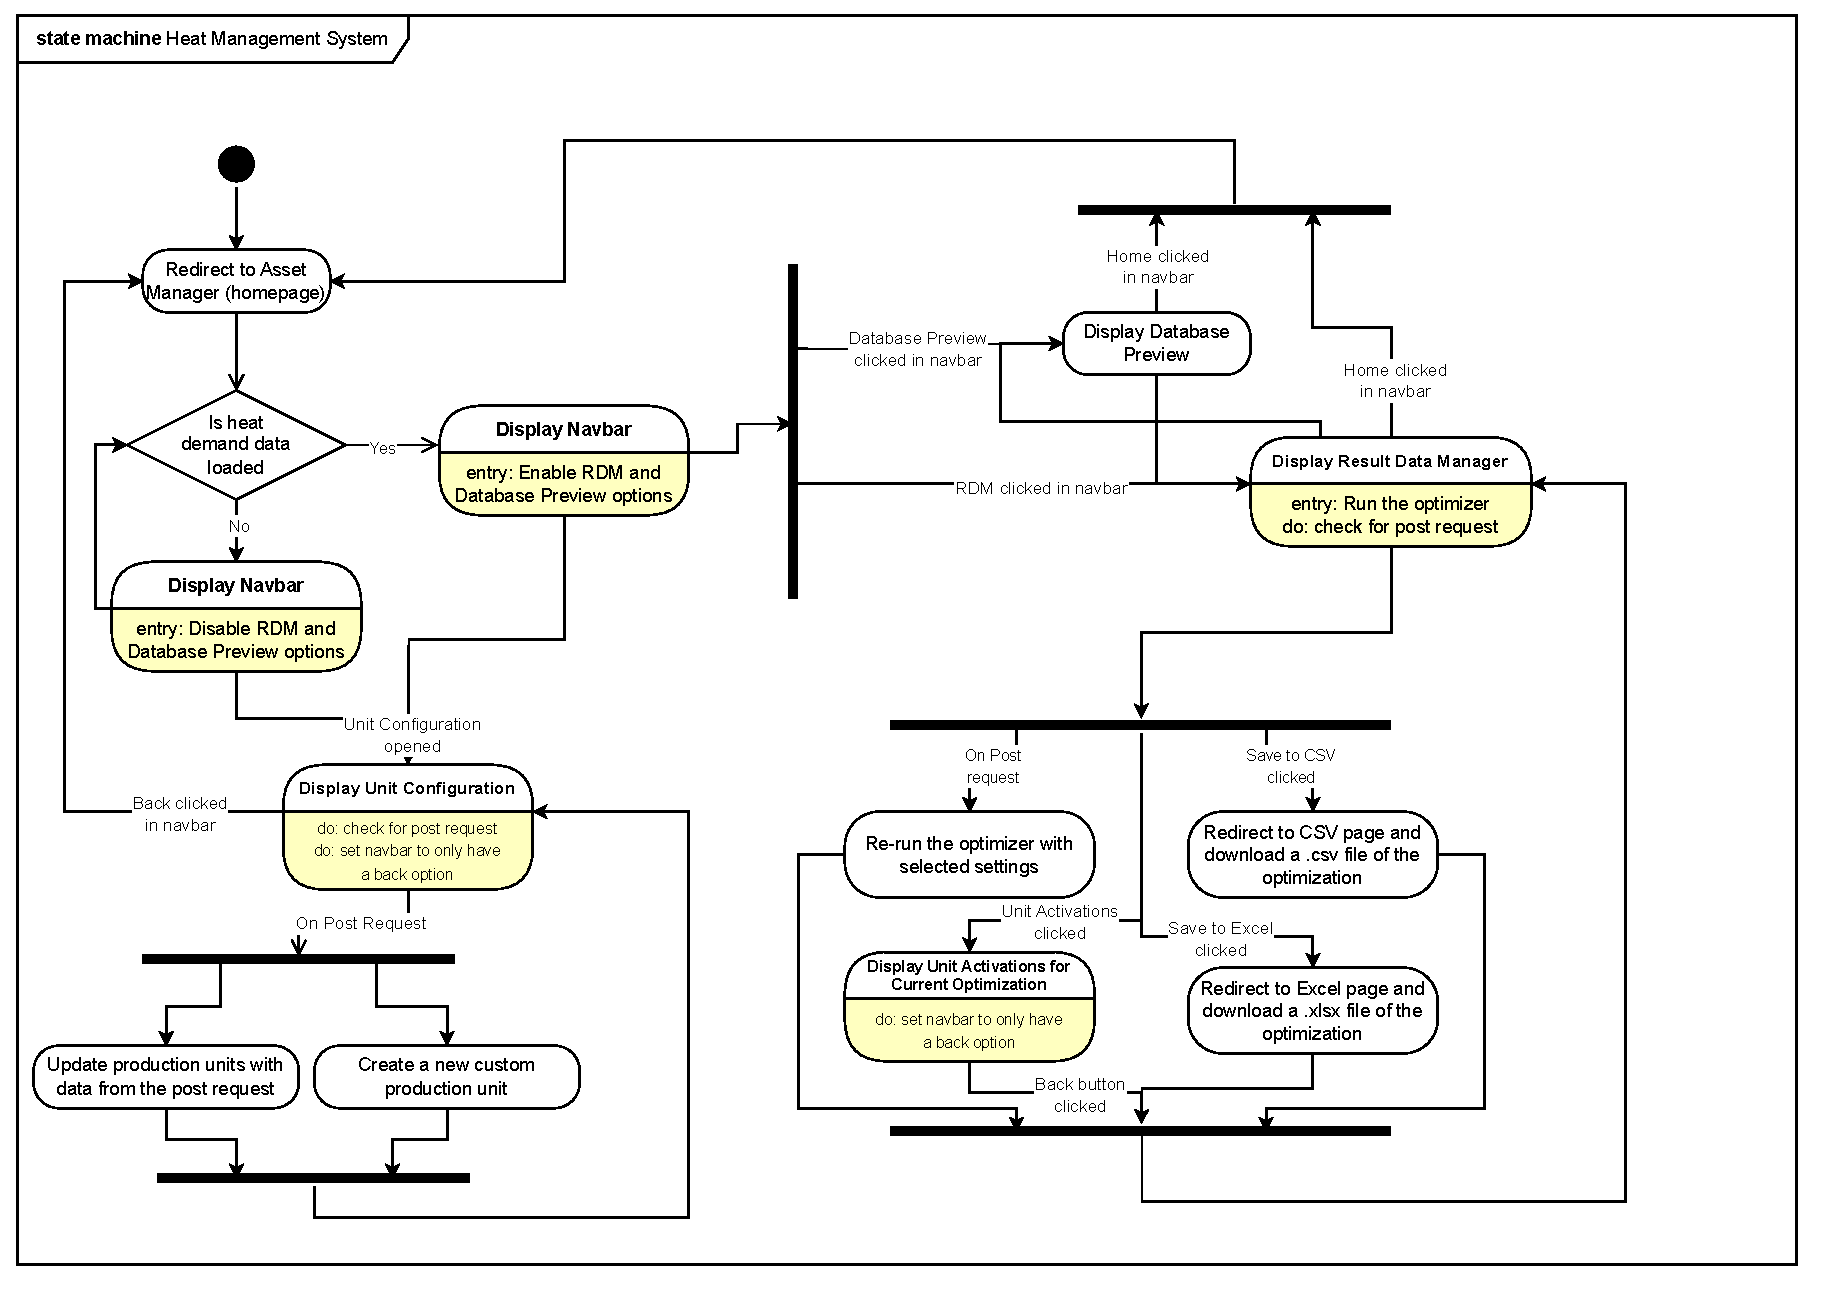
\includepdf[pages=-]{Resources/SP2-state-machine.pdf}


\subsection*{Database Design}
\label{sec:database}
Before diving into the program architecture the in-memory database solution offered by Razor Pages must first be mentioned.
In order to achieve data persistance while switching in between pages in a Razor Pages project, a database must be used. 
Since we did not want to go too far out of the scope of the project, we decided not to use a dedicated database solution
like a MySQL or MSSQL Server for this project, expecially because the team has not had any database modeling courses
yet. Instead we chose a middle-ground, which is the before mentioned in-memory database. This soultion offers similar functionality
to a real database, with the comfort of running in the program's memory, which eliminates potential connection, authentication
privilege and/or security risks and issues connected with using databases. To represent the applications data storage sytstem
the group devised an improvised custom uml diagram inspired by other standardized database diagrams. It can be seen below, together with
explanation for each of the tables.

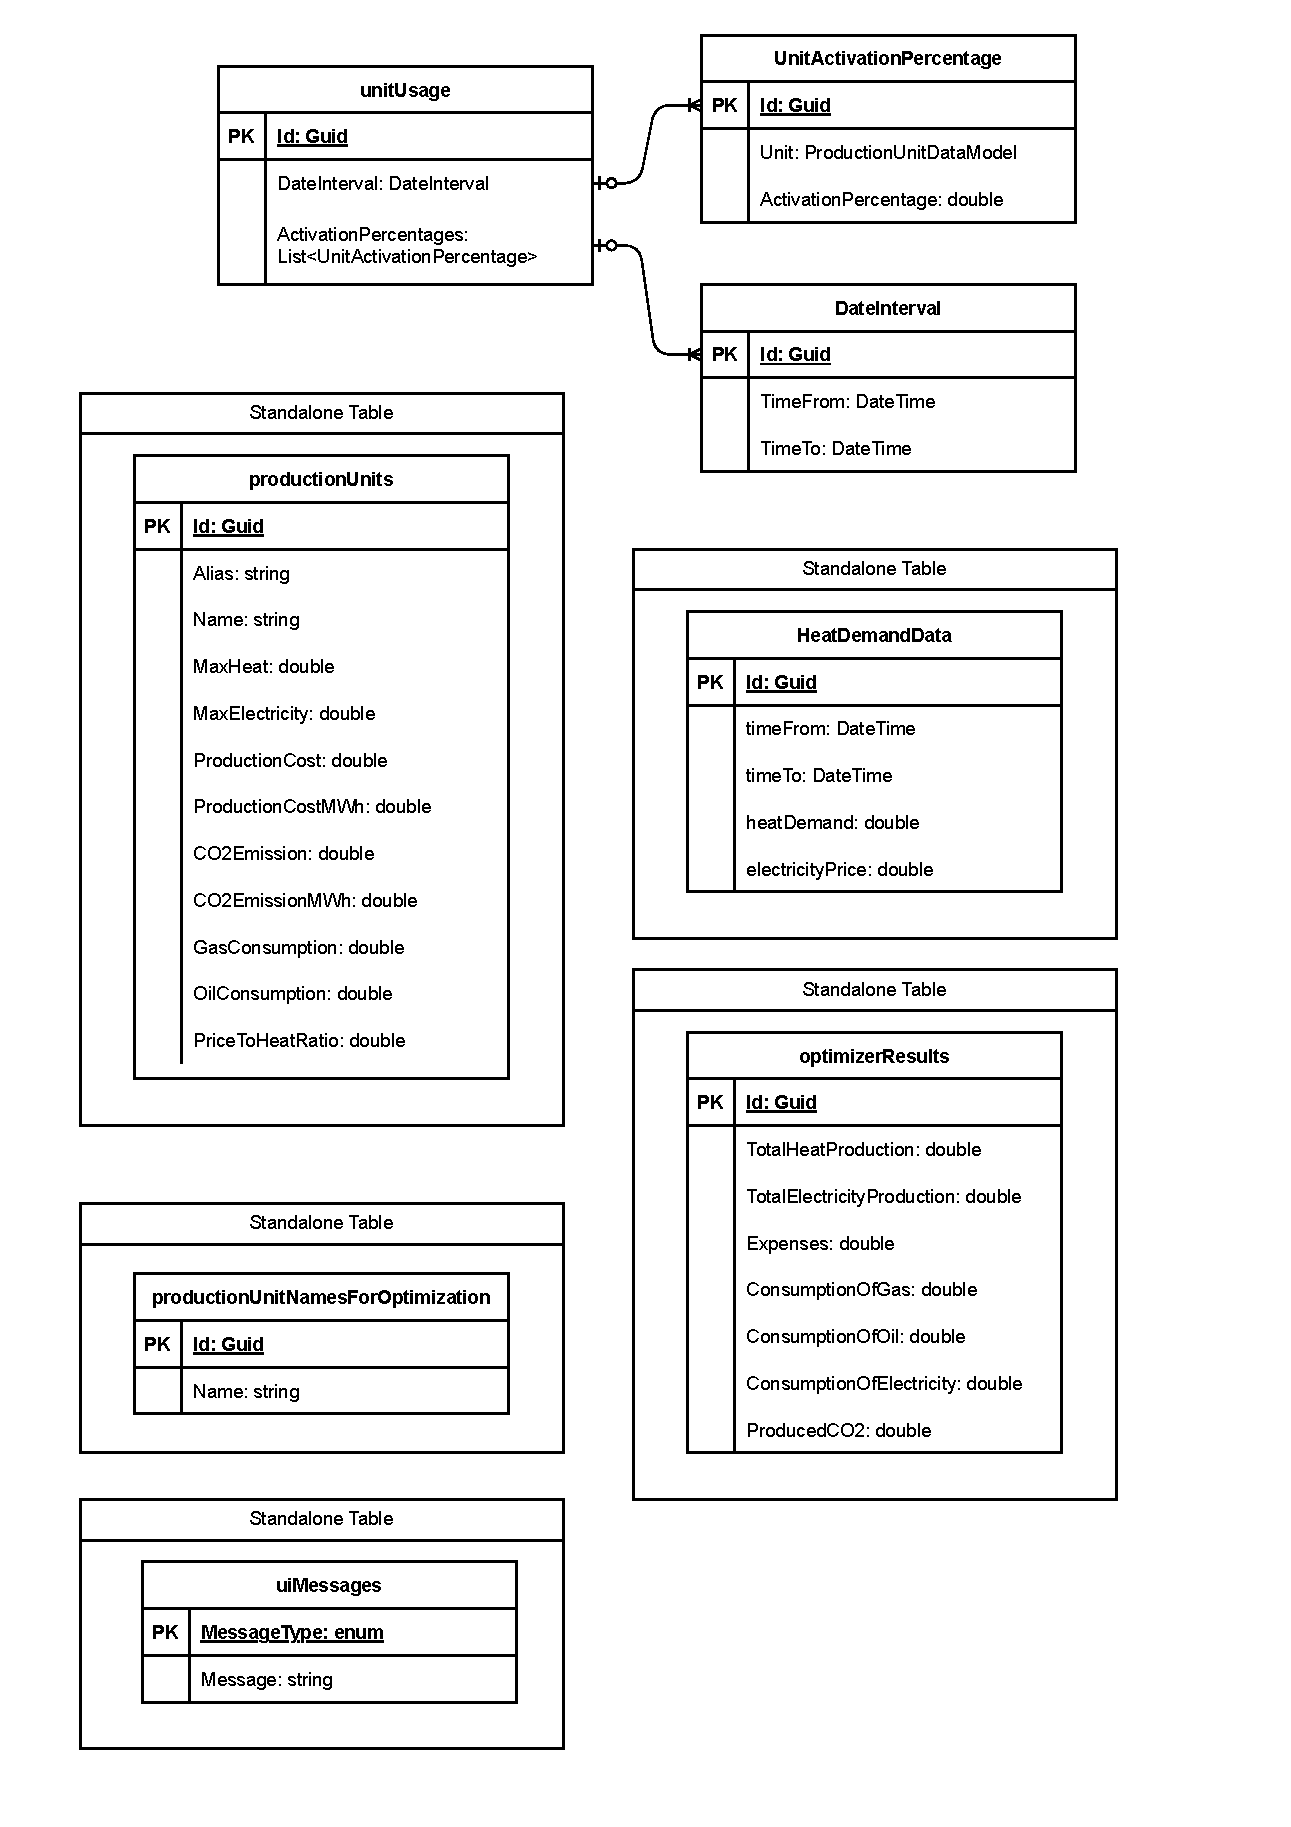
\includepdf[pages=-]{Resources/SP2-database-diagram.pdf}

The database does not fully comply to database system standards. 
We do see the limitations and flaws of this design choice, such as the lack of connections between tables and the 
lack of foreign keys inside of each table. Instead some fields in the tables use custom class data types for ease of use. Despite the flaws
of using DbSets, we found that their functionality was sufficient for the scope of the project. It is also worth to mention, that due
to our lack of experience with Razor Pages, we were unsure of how DbSets and in-memory data structures function. Because of that in the
middle of development the database had to be refactored from a more json-like data storage structure to one that complies
with standards enforced by DbSets, such as using Primary Keys. It is because of this process that we ended up having a mixture of both structures.
The most crucial tables found within the programs database are the \textit{productionUnits} and \textit{HeatDemandData}. As the names suggests
they contain data that is needed for the application's main functionality - calculating optimized production unit usage results for 
the inputted heat demand for each timeframe. Some of the properties inside of \textit{productionUnits} are additions from the team, such as
\textit{ProductionCostMWh} and \textit{CO2EmissionMWh}, which made it easier to remember how to calculate final optimization results, and
\textit{PriceToHeatRatio}, which also was a helper variable in optimization calculations.
When it comes to storing the results from the optimizer for later display or download, the \textit{unitUsage} and \textit{optimizerResults} tables were used.
We think their names explain their functionality sufficiently.
Lastly, the \textit{uiMessages}, as the name suggests stores messages for the user that may appear in the user interface under certain conditions, such as 
confirmation of a successful data upload or an error during the optimization process.
These messages have to be stored in a database, because of how user input works in Razor Pages. The only way the team found to obtain user input is through
post requests, which only make impact on the interface after a page redirect, which would reset the pages memory and lose the message intended for display.
That is why for these messages to persist it is important to have a place to save them before the redirect.


\subsection*{Code Architecture}
\label{sec:code}
With the database covered, we can shift our focus towards the rest of the codebase. Any issues, bugs or problems encountered
by the group during the development/implementation phase of the project will be \underline{underlined} in this subsection of the report.
We shall start in the same place as the program's structure: \textit{Program.cs}. This file mostly contains
automatically generated Razor Pages setup code for every built-in feature to work correctly, but it is also where one of the first problems started.
\underline{Culture Info} was a common problem across all groups working on this project in this semester, and it definitely caused some issues for us as well,
like incorrect DateTime variable parsing, incorrect decimal separator detection, errors with reading data from files and incorrect data display.
Fortunately manually setting the user's DefaultThreadCurrentCulture and DefaultThreadCurrentUICulture to the Danish CultureInfo
was an easy fix that solved most of these problems. From this code file, the Razor Pages applications gets built and the user gets redirected
to the \textit{Index.cshtml} page with the Navbar and DataUpload ViewComponents overlayed on top of it, which we will come back to shortly.
The group chose to create both component and class diagrams to explain how the code is designed. The component diagram helps us break down
the program into the components from the project's requirements, and clarify in which location each component is implemented.
This diagram also plays a part in explaining the interactions between each component, and the class diagram is able to complete this explanation,
as well as go more in depth for each component, breaking them down into individual classes. The component diagram can be seen below.

% Include the finished component diagram here

Following the component hierarchy we will cover the \textbf{Source Data Manager} next. The class diagrams facilitating this explanation
can be seen below this paragraph. Our implementation of this component makes it handle the most important interaction between the program
and the database, which is loading user input or pre-loaded data and deleting that data. The component itself is an 
implementation of the \textit{IDatabaseManager} interface, which was used to reinforce the SOLID principles within our codebase,
decouple dependencies, make the code less brittle and more expandable. The main property of \textbf{Source Data Manager} is \textit{\_context},
which will appear in most other components, and is essentially a reference to the in-memory database. \textit{SourceDataDbContext}, which
implements the \textit{DbContext} Interface is the class that contains the in-memory database. It uses class data models such as 
\textit{HeatDemandDataModel}, \textit{ProductionUnitDataModel}, \textit{OptimizerUnitNamesDataModel}, \textit{UnitUsageDataModel},
\textit{UiMessagesDataModel} and \textit{OptimizerResultsDataModel} for data storage. The other properties it contains have custom get and set methods
defined which interact with their respective DbSets, and serve as quick references to specific items from the database that are widely used throughout the program.
This is a result of \underline{major database} \underline{refactor}, before which these properties were preset in the \textbf{Source Data Manager} component.
In order to avoid merge conflicts and errors these properties were kept but puerly as references to the database, which is where
C\#'s feature of custom property getters and setters came in really handy.
Moving onto the \textbf{Asset Manager} component, which uses the \textit{IndexModel.cshtml.cs} class as it's code-behind. As mentioned
previously, this is the Homepage of the program, it contains a reference to the database, OnGet and OnPost methods for handling user
input.
In this component, we also made use of Razor Pages' View Component feature, which essentially allowed us to display a page within
another page, which helped break up the code into more manageable chunks and work on different parts of the page without interfering with each other.
The only two View Components in the program are:
\begin{itemize}
  \item DataUploadView - a page that either calls \textbf{Source Data Manager} to load in pre-provided heat demand data,
  or accepts a file uploaded by the user, while checking if its format and extension is correct.
  \item PageNavigationView - as the name suggests, it is an overlay that allows the user to navigate through the program, namely
  to three components: \textbf{Asset Manager}, \textbf{Result Data Manager} and \textbf{Database Preview}. The navigation bar is displayed
  in each mentioned component.
\end{itemize}
The \textbf{Asset Manager} also gives access to the \textbf{Production Unit Configuration} component. This is where the user
can configure properties of pre-existing or custom added production units. All of the user input is again handled in the OnGet and OnPost methods
with the aid of the \textit{PUCButtonRequest} class, which allows the OnPost request to recognize which button in the UI was pressed
and to react accordingly. Unit creation, updating and deletion processes use unit IDs from the \textit{ProductionUnitDataModel} class
to make sure changes occur to the right unit, thanks to Guid ensuring each Production Unit record in the database has a unique ID.
Obtaining the new parameters for chaning a picked production unit is handled thorugh binding the \textit{formProductionUnit} property, which is
a technique used also in other pages when handling user input. This is also where an issue came up connected with
\underline{Culture Info}, that was not solved in \textit{Program.cs}, which were the decimal separators for number inputs.
This is why a custom \textit{DoubleModelBinder} was written, to convert HTML form input's values to variables of type \textit{double}
no matter if they used a dot or a comma as their decimal separator. A safety check was also implemented, so that a production
unit's Alias property has to be unique, to eliminate potential errors with the optimization process, which will be covered soon.

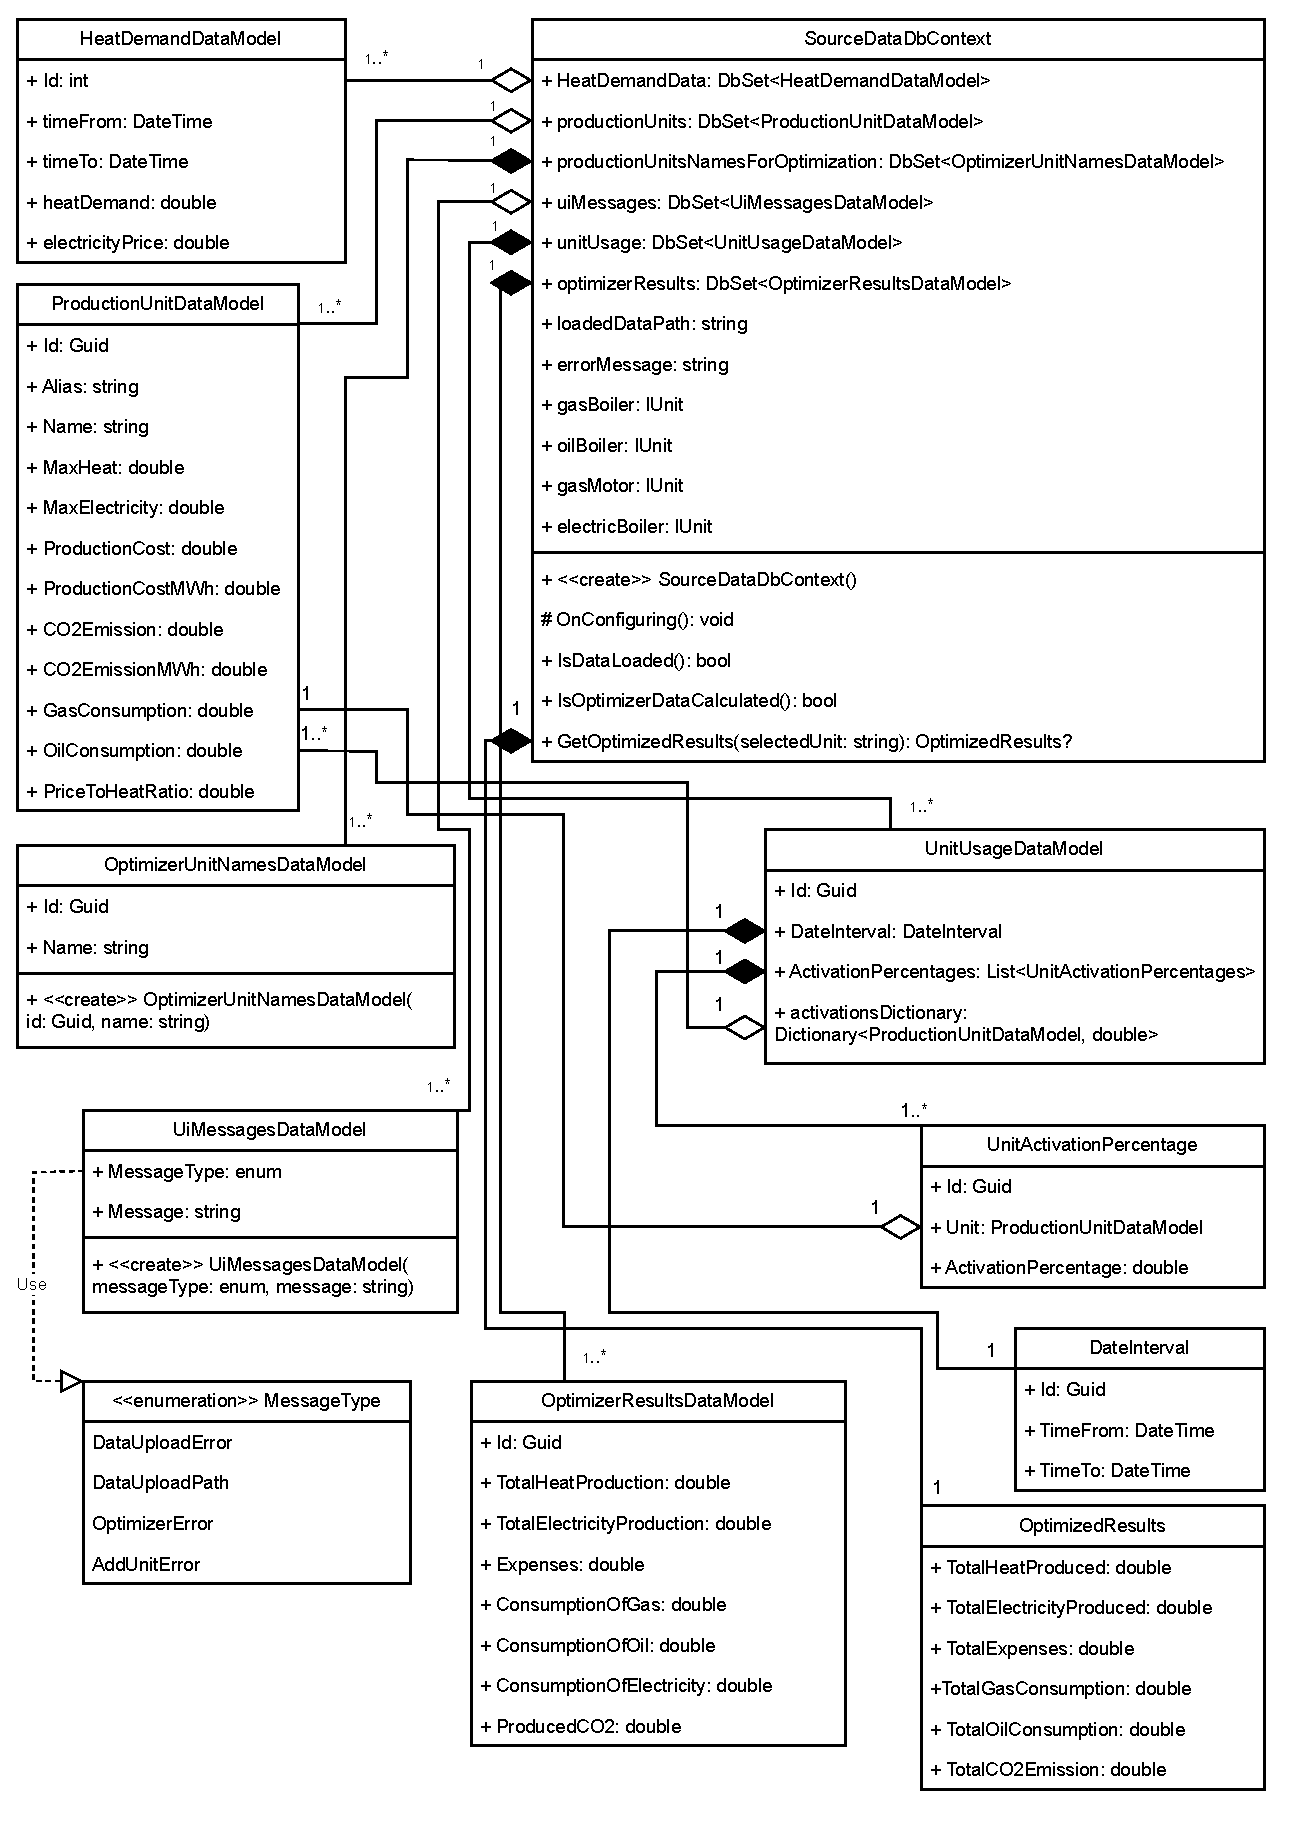
\includepdf[page={4, 1}]{Resources/SP2-class-diagrams.pdf}

Back in \textbf{Asset Manager}, the navbar allows the user to navigate to the \textbf{Result Data Manager} and \textbf{Database Preview}
components. The latter does not contain any distinguishing code, and was covered entirely in the subsection \hyperref[sec:appflow]{Application Flow}.
The \textbf{Result Data Manager}, on the other hand, is the most substancial component of the whole application. The code-behind for its page
is in \textit{ResultDataManagerModel.cshtml.cs}. It contains the usual reference to the database, but a thing that stands out
are the two IUnit Lists and the IUnit Interface itself. Firstly, the program contains both a IUnit Interface and a ProductionUnitDataModel parent class
for production units, which are used interchangeably, because of a \underline{DbSet issue}. At one point in the development
when trying to access one of the feature of DbSets, it turned out that a DbSet cannot be of an interface type. At that point, the IUnit
interface was used extensively within the codebase and there was not enough time to make the changes necessary, so a band-aid fix was applied, with which
the ProductionUnitDataModel class was created. The \textbf{Result Data Manager} also hosts the \textbf{Optimizer}
component, which consists of the KOptimizer, SOptimizer, GeneticAlgorithm (The Neural Network Optimizer) (and WorstScenarioOptimizer with RandomOptimizer, which
are used solely as comparison data for some of the graphs). Multiple Optimizer implementations are a result of one of the
\hyperref[sec:sprints]{Sprints} the team carried out, where everyone worked on an implementation and at the end the best one was chosen.
The main optimizer that the application uses is the KOptimizer, which is also referred to as the Standard Optimizer. It is a simple
Greedy Algorithm implementation that judges which production units are the most cost effective for each timeframe, and uses 
them to produce as much heat as possible until the demand is met. An outlier to the goal of our optimizer sprint was the Neural Network Optimizer,
which was too good of an idea to pass up on, while begin to risky to be the only optimization algorithm, so we decided to use both.
The explanation on how it is implemented can be found in \hyperref[sec:nnexplanation]{Chapter 5c}.
The Optimization Process has 3 main configuration options to consider before re-running it, which were also mentioned in \hyperref[sec:appflow]{Application Flow}.
This configuration is handled in the OnPost method of ResultDataManagerModel. It is important to mention, that due to \underline{allowing}
\underline{the user to choose their own production unit scenario}, each \textbf{Optimizer} implementation had to have a built-in check to
make sure that the production units provided can even meet the heat demand. If that is not the case, the uiMessages
DbSet is used in the database to display an error message to the user.
Additionally, this option meant that we needed to store all of the production units and the production units selected for 
the optimization process by the user at the same time. This is where a second \underline{problem with DbSets} came up.
Razor Pages does not seem to allow for two DbSets of the same type to exist within one database, instead
merging them into one singular DbSet if that was the case, resulting in duplicate key value errors. A workaround had to be implemented.
This is why the OptimizerUnitNamesDataModel exists, which stores just the production unit aliases, which are then matched
with the prodcution units in the productionUnits DbSet and passed into the \textbf{Optimizer}. This is also why the \textbf{Unit Configuration}
component makes sure that each alias is unique.
Once the optimization process is finished, the \textbf{Result Data Manager} saves the outputs to the database using
the UnitUsageDataModel and OptimizerResultsDataModel classes. This is what later allows the ExcelWriter and CSVWriter classes
to access this data, convert it to their own respective formats, and redirect the user to a file download page.
Lastly, \textbf{Result Data Manager} also hosts the \textbf{Unit Activations} component, which in similar fashion
as the \textbf{Database Preview}, was covered in \hyperref[sec:appflow]{Application Flow}.

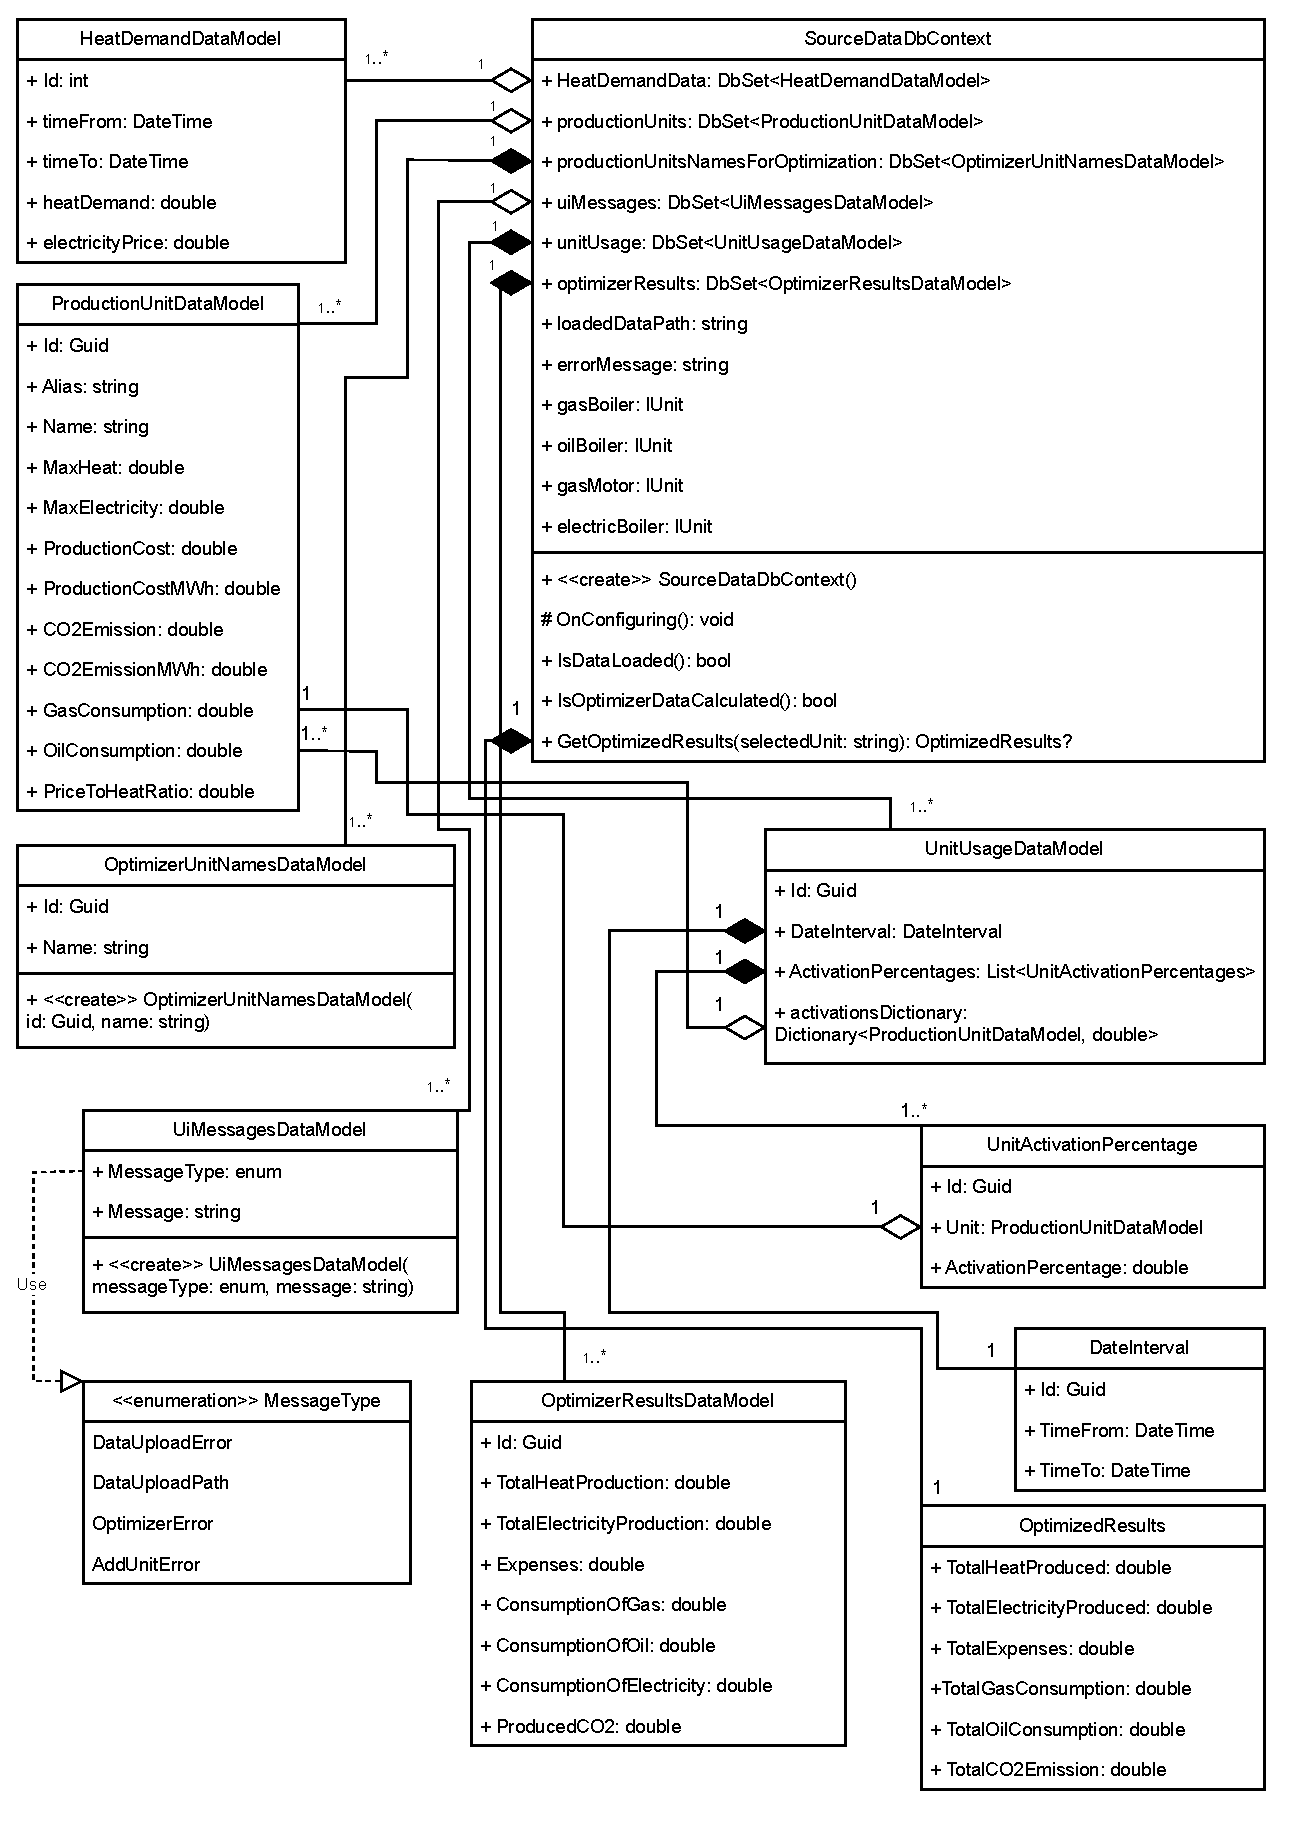
\includepdf[page={3, 2}]{Resources/SP2-class-diagrams.pdf}

% Chapter 4b
\section{Simple Design}
Simple design yapping goes here

% Chapter 4c
\section{Incremental Design}
Incremental Design yapping goes here

% Chapter 4d
\section{Refactoring}

Most of the group did not have much experience in this process because most of the assignments we were being given
were not on a large enough scale to consider restructuring code throughout their development - the tasks and functionality
were finished long before poor code design could become a problem.
The scope and timespan of this project was much larger, therefore the we decided that refactoring should play a considerable
role in our development. Somewhat to our surprise, refactoring felt quite natural, especially since this was the team's first
project with Razor Pages, the more we learned about the framework and the more we understood, the more we saw of what 
could be implemented better, improved or discarded. Some features of the application even required code refactors, because the
foundation of the program could not have facilitated them beforehand due to our initial poor understanding of the framework.
It is fair to say that a considerable amount of development time was dedicated solely to code refactoring and it very much 
paid off in the long run. We found that thanks to continuous code maintenance and refactors, the source code became simpler, cleaner,
easier to understand and more expandable. Frequent refactoring also strengthened the code's structure, making it less brittle as well
as eliminating a sizeable amount of bugs and vulnerabilities the team was struggling with, which could be called a happy accident.
A great example of refactoring done by the group are the database refactors described in \hyperref[sec:database]{Datbase Design}
and \hyperref[sec:code]{Code Architecture}. Storing variables the traditional, which is what we have been doing for all our previous
assignments just did not work with Razor Pages, thus we needed to shift more to a database mindset. The first 'code smell' that suggested
it was a bug with displaying conditional ui messages for the user, they would show up once but after a refresh disappear, simply because
they were not stored in a database.
Another instance of refactoring in development was handling the output data from the \textbf{Optimizer} component. At first
every component that wanted to access it had to get the appropriate properties from the object instance itself. This created and issue
when it came time to implement downloading this data to the user's device. Since the user needed to be redirected to a different page,
we could not pass over the object reference, so a change was made to store the results in the database. With that also came another
refactor to the structure of the \textbf{Optimizer's} output data, which was simplified and made compatible with storing in the DbSet
data structure. This was a prime example of how refactoring made it easier to work with the code and simplified the underlying
logic of a component.

Code refactoring was tremendously benefitial in the implementation phase of our application, and we will most definitely
keep this practice in the future, maybe even putting more focus on it.

% Chapter 4e
\section{Test-Driven Development}
Test-Driven Development yapping goes here

% Chapter 4f
\section{Unit Testing}
Unit Testing yapping goes here

% Chapter 4g
\section{Pair Programming}
Pair Programming yapping goes here

% Chapter 4h
\section{Code Review}
Code Review yapping goes here

% Chapter 5
\chapter{Conclusion and Group's Reflections}
Conclusion chapter goes here

% Chapter 5a
\section{Working on a common project with other groups}
5a yapping goes here

% Chapter 5b
\section{What went well and not so well with the group's specific set of tasks}
5b yapping goes here

% Chapter 5c
\section{Specific contributions of each team member}
5c yapping goes here

\label{sec:nnexplanation} %explain how the neural network optimizer works here

\section{Future actions to prevent problems and difficulties faced during the project}
5d yapping goes here


\end{document}